\documentclass[a4paper,11pt,twoside]{ThesisStyle}

\include{formatAndDefs}
\usepackage{listings}
\renewcommand{\lstlistingname}{Code source}
\usepackage{color}
\definecolor{lightgray}{rgb}{.9,.9,.9}
\definecolor{darkgray}{rgb}{.4,.4,.4}
\definecolor{purple}{rgb}{0.65, 0.12, 0.82}
\definecolor{ocher}{rgb}{1, 0.5, 0} % #FF7F00 -> rgb(239, 169, 0)
\definecolor{green}{rgb}{0, 0.5, 0} % #007C00 -> rgb(0, 124, 0)
\definecolor{olive}{rgb}{0.17,0.59,0.20}
\definecolor{brown}{rgb}{0.69,0.31,0.31}

\lstdefinelanguage{CSS}{
  keywords={color,background-image:,margin,padding,font,weight,display,position,top,left,right,bottom,list,style,border,size,white,space,min,width, transition:, transform:, transition-property, transition-duration, transition-timing-function},	
  sensitive=true,
  morecomment=[l]{//},
  morecomment=[s]{/*}{*/},
  morestring=[b]',
  morestring=[b]",
  alsoletter={:},
  alsodigit={-}
}
\lstdefinelanguage{JavaScript}{
  morekeywords={typeof, new, true, false, catch, function, return, null, catch, switch, var, if, in, while, do, else, case, break},
  morecomment=[s]{/*}{*/},
  morecomment=[l]//,
  morestring=[b]",
  morestring=[b]'
}
\lstdefinelanguage{HTML5}{
  language=html,
  sensitive=true,	
  alsoletter={<>=-},	
  morecomment=[s]{<!-}{-->},
  tag=[s],
  otherkeywords={
  % General
  >,
  % Standard tags
	<!DOCTYPE,
  </html, <html, <head, <title, </title, <style, </style, <link, </head, <meta, />,
	% body
	</body, <body,
	% Divs
	</div, <div, </div>, 
	% Paragraphs
	</p, <p, </p>,
	% scripts
	</script, <script,
  % More tags...
  <canvas, /canvas>, <svg, <rect, <animateTransform, </rect>, </svg>, <video, <source, <iframe, </iframe>, </video>, <image, </image>, <header, </header, <article, </article
  },
  ndkeywords={
  % General
  =,
  % HTML attributes
  charset=, src=, id=, width=, height=, style=, type=, rel=, href=,
  % SVG attributes
  fill=, attributeName=, begin=, dur=, from=, to=, poster=, controls=, x=, y=, repeatCount=, xlink:href=,
  % properties
  margin:, padding:, background-image:, border:, top:, left:, position:, width:, height:, margin-top:, margin-bottom:, font-size:, line-height:,
	% CSS3 properties
  transform:, -moz-transform:, -webkit-transform:,
  animation:, -webkit-animation:,
  transition:,  transition-duration:, transition-property:, transition-timing-function:,
  }
}
\lstset{
   %backgroundcolor=\color{lightgray},
   extendedchars=true,
   basicstyle=\footnotesize\ttfamily,
   showstringspaces=false,
   showspaces=false,
   numbers=left,
   numberstyle=\tiny,
   numbersep=9pt,
   tabsize=2,
   breaklines=true,
   showtabs=false,
   captionpos=b,
   frame=single,
   keywordstyle=\color{blue}\bfseries,
   ndkeywordstyle=\color{green}\bfseries,
   identifierstyle=\color{black},
   commentstyle=\color{purple}\ttfamily,
   stringstyle=\color{brown}\ttfamily,
}

\usepackage{titlesec}
\usepackage{changepage}
\usepackage{tabularx}
\usepackage{hyperref}
\usepackage{graphicx}

\usepackage{listings}
\usepackage{color}
\definecolor{lightgray}{rgb}{.9,.9,.9}
\definecolor{darkgray}{rgb}{.4,.4,.4}
\definecolor{purple}{rgb}{0.65, 0.12, 0.82}
\definecolor{ocher}{rgb}{1, 0.5, 0} % #FF7F00 -> rgb(239, 169, 0)
\definecolor{green}{rgb}{0, 0.5, 0} % #007C00 -> rgb(0, 124, 0)
\definecolor{olive}{rgb}{0.17,0.59,0.20}
\definecolor{brown}{rgb}{0.69,0.31,0.31}

\lstdefinelanguage{CSS}{
  keywords={color,background-image:,margin,padding,font,weight,display,position,top,left,right,bottom,list,style,border,size,white,space,min,width, transition:, transform:, transition-property, transition-duration, transition-timing-function},	
  sensitive=true,
  morecomment=[l]{//},
  morecomment=[s]{/*}{*/},
  morestring=[b]',
  morestring=[b]",
  alsoletter={:},
  alsodigit={-}
}
\lstdefinelanguage{JavaScript}{
  morekeywords={typeof, new, true, false, catch, function, return, null, catch, switch, var, if, in, while, do, else, case, break},
  morecomment=[s]{/*}{*/},
  morecomment=[l]//,
  morestring=[b]",
  morestring=[b]'
}
\lstdefinelanguage{HTML5}{
  language=html,
  sensitive=true,	
  alsoletter={<>=-},	
  morecomment=[s]{<!-}{-->},
  tag=[s],
  otherkeywords={
  % General
  >,
  % Standard tags
	<!DOCTYPE,
  </html, <html, <head, <title, </title, <style, </style, <link, </head, <meta, />,
	% body
	</body, <body,
	% Divs
	</div, <div, </div>, 
	% Paragraphs
	</p, <p, </p>,
	% scripts
	</script, <script,
  % More tags...
  <canvas, /canvas>, <svg, <rect, <animateTransform, </rect>, </svg>, <video, <source, <iframe, </iframe>, </video>, <image, </image>, <header, </header, <article, </article
  },
  ndkeywords={
  % General
  =,
  % HTML attributes
  charset=, src=, id=, width=, height=, style=, type=, rel=, href=,
  % SVG attributes
  fill=, attributeName=, begin=, dur=, from=, to=, poster=, controls=, x=, y=, repeatCount=, xlink:href=,
  % properties
  margin:, padding:, background-image:, border:, top:, left:, position:, width:, height:, margin-top:, margin-bottom:, font-size:, line-height:,
	% CSS3 properties
  transform:, -moz-transform:, -webkit-transform:,
  animation:, -webkit-animation:,
  transition:,  transition-duration:, transition-property:, transition-timing-function:,
  }
}
\lstset{
   %backgroundcolor=\color{lightgray},
   extendedchars=true,
   basicstyle=\footnotesize\ttfamily,
   showstringspaces=false,
   showspaces=false,
   numbers=left,
   numberstyle=\tiny,
   numbersep=9pt,
   tabsize=2,
   breaklines=true,
   showtabs=false,
   captionpos=b,
   frame=single,
   keywordstyle=\color{blue}\bfseries,
   ndkeywordstyle=\color{green}\bfseries,
   identifierstyle=\color{black},
   commentstyle=\color{purple}\ttfamily,
   stringstyle=\color{brown}\ttfamily,
}
\usepackage[nomain,acronym,xindy,toc]{glossaries}
\makeglossary
\usepackage[xindy]{imakeidx}
\makeindex

\usepackage{epstopdf}
\usepackage[T1]{fontenc}
\usepackage[utf8]{inputenc}
\usepackage[francais]{babel}


\newcommand{\fwshort}{RSnap}
\newcommand{\fwlong}{Une plateforme web pour apprendre le "raisonnement informatique" aux jeunes du primaire et secondaire}
\newcommand{\HRule}{\rule{\linewidth}{0.5mm}}
\newcommand{\hRule}{\rule{\linewidth}{0.1mm}}
\def \doctitle {Une plateforme web pour apprendre le "raisonnement informatique" aux jeunes du primaire et secondaire}
\def \docsubtitle {}
\def \doccourssigle{LINGI2990}
\def \doccourstitle{Master Thesis}
\def \docauthor {Gaetan {\sc Collart}\\\emph{Année :} INFO 22 MS\\\emph{Noma :} 66-20-07-00 \and Simon {\sc Claessens}\\\emph{Année :} INFO 22 MS\\\emph{Noma :} 31-06-07-00}
\def \docprofessor{Chantal \textsc{Poncin} \and Pierre Schaus}
%\def \docassistant{Nicolas \textsc{Cardozo Alvarez}}

\author{Gaetan {\sc Collart}\\\emph{Année :} INFO 22 MS\\\emph{Noma :} 66-20-07-00 \and Simon {\sc Claessens}\\\emph{Année :} INFO 22 MS\\\emph{Noma :} 31-06-07-00}
\title{Une plateforme web pour apprendre le "raisonnement informatique" aux jeunes du primaire et secondaire}

\usepackage{mdwlist} %reduce itemize item spacing
\usepackage{placeins} 

\usepackage[plain]{fancyref}
\def\fref{\Fref} % treat all \frefs as \Frefs
% Define 'lst' delimiter for fancyref
\newcommand*{\fancyreflstlabelprefix}{lst}
\newcommand*{\Freflstname}{\lstlistingname}
\newcommand*{\freflstname}{\MakeLowercase{\lstlistingname}}
\Frefformat{vario}{\fancyreflstlabelprefix}%
 {\Freflstname\fancyrefdefaultspacing#1#3}

\frefformat{vario}{\fancyreflstlabelprefix}%
 {\freflstname\fancyrefdefaultspacing#1#3}
\Frefformat{plain}{\fancyreflstlabelprefix}%
 {\Freflstname\fancyrefdefaultspacing#1}
\frefformat{plain}{\fancyreflstlabelprefix}%%
 {\freflstname\fancyrefdefaultspacing#1}





\usepackage{wrapfig}
%\includeonly{titlepage}
%\includeonly{titlepage,content/androidinjava/androidjava}
%\includeonly{titlepage,content/Intro/abstract,content/Intro/thanks,content/Intro/intro}
%\includeonly{titlepage,content/Intro/abstract,content/Intro/intro,content/conclusion/futurework,content/conclusion/conclusion}
%\includeonly{content/cityvisit/cityvisit,content/cityvisit/data}
%\includeonly{content/scopj/scopj}
%======================
%	DOCUMENT
%======================
%http://en.wikibooks.org/wiki/LaTeX/Glossary
\newacronym{ddye}{D}{donor dye, ex. Alexa 488}
\newacronym[description={\glslink{r0}{F\"{o}rster distance}}]{R0}{$R_{0}$}{F\"{o}rster distance}
\newglossaryentry{r0}{name=\glslink{R0}{\ensuremath{R_{0}}},text=F\"{o}rster distance,description={F\"{o}rster distance, where 50\% ...}, sort=R}
\newglossaryentry{kdeac}{name=\glslink{R0}{\ensuremath{k_{DEAC}}},text=$k_{DEAC}$, description={is the rate of deactivation from ... and emission)}, sort=k}
\begin{document}
%\dominitoc


\maketitle
%\input{titlepage}

\pagenumbering{arabic}

\section*{Abstract}

\section{Remerciements}
\newpage
%\faketableofcontents
\tableofcontents


%\mainmatter
\section{Introduction}

%==========================
%       PART 1
%==========================
\chapter{Théorie}
Dans cette section nous allons présenté les prérequis et un état des lieux de l'apprentissage de la programmation aux enfant dans le monde. Nous avons en premier les prérequis et SNAP BYOB qui est l'application que nous avons réutiliser. Ensuite nous analyserons les autres initiatives similaire à celle de ce travail. Pour conclure nous positionnerons le projet RSNAP par rapport à ce qui est déjà existant et expliqué dans les points précédent.

\chapter{Connaissances nécessaires}
Ce chapitre commencera par présenter de manière succincte les prérequis pour pouvoir suivre ce document. Ensuite, une description plus technique présentera les outils utilisés.

\section{Prérequis}
Les connaissances nécessaires à la bonne compréhension de ce travail vont être développées dans cette partie.

\paragraph{Snap!}
Commençons par la partie portant sur Snap! BYOB. Cette application est implémentée en JavaScript. Donc, de bonnes connaissances dans ce langage de programmation seront un atout pour comprendre les apports et modifications de la version de départ. Des connaissances en XML et JSON seront également un plus pour toutes les fonctions d'importation et d'exportation.

\paragraph{Ruby on Rails}
La plateforme web, elle est implémentée en Ruby on Rails qui est le framework le plus utilisé pour la création de site web en Ruby. Ce framework est un atout car il permet de créer facilement des sites sur une architecture de type modèle-vue-contrôleur. Rails se base sur des conventions au lieu de se baser sur des configurations. Cela permet d'alléger considérablement le nombre de lignes nécessaires pour la création d'un site web. Ce framework étant basé sur Ruby, il permet l'usage des gems Ruby. Un gems est une bibliothèque logicielle qui permet d'avoir facilement des fonctionnalités supplémentaires. Plus de détails techniques seront donnés dans la suite de ce chapitre \ref{techno}. %TODO ajouter gem au glossaire

\paragraph{Pédagogie}
Pour l'apprentissage de la programmation aux jeunes, des notions de pédagogie sont également nécessaires. 
Les programmes d'apprentissages existants permettent de définir pour chaque année d'étude, les concepts considérés comme acquis par les élèves. La communication avec les jeunes demande un vocabulaire adapté. Tout ceci s'avère important pour les choix de design d'interface. Par exemple, suivant leur âge, les jeunes ne seront pas stimulés par les mêmes images ou couleurs. %TODO revoir ce chapitre

\subsection{Logiciel utilisé}
\subsubsection{Snap!}
\url{http://snap.berkeley.edu/SnapManual.pdf}
Cet partie va donner un aperçu de l'application réutilisée dans ce travail, à savoir Snap!. Comme dit précédemment, cette application est réalisée en JavaScript. La présentation de Snap! va se diviser en plusieurs partie. La première expliquera les différents types de blocs et comment ils sont implémentés. L'exécution d'un programme est l'étape suivante. Enfin, il sera présenté comment l'application affiche les différents éléments la constituant.

\paragraph{Blocs}
Il existe plusieurs type de blocs qui constitue un programme Snap!. Sur l'exemple de programme \ref{fig:software_used_script}, les différents types blocs disponible sont présentés.
\begin{figure}
  \begin{center}
    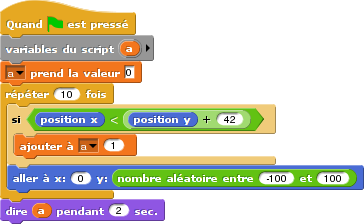
\includegraphics[width=0.5\textwidth]{content/4-theory/2-related_work/images/script}
    \caption{Exemple de programme Snap!}
    \label{fig:software_used_script}
  \end{center}
\end{figure}

\subparagraph{Commande}
Le type principal de bloc est \texttt{commande}. Ces blocs peuvent être compris comme étant des procédures. En effet, les blocs exécutes une ou plusieurs opérations sur le système en fonction des paramètres passés. Ces différents blocs doivent se baser soit sur une implémentation JavaScript pour les commandes élémentaires, soit être une composition de commandes pour fournir une commande plus complexe et/ou abstraite.

Dans l'exemple \ref{fig:software_used_script}, ce sont tout les blocs qui on la forme d'une pièce de puzzle. On peut voir que l'on a une succession de commandes qui crée un script. Les commandes ont plusieurs couleurs suivant la catégorie à laquelle elles appartiennent : mouvement, apparence, contrôles, variable, etc\ldots

\subparagraph{Reporter}
Les reporters sont des fonctions. En effet, ils retournent une valeur. Ils sont toujours utilisés en temps que paramètres d'un autre bloc. La plupart des reporter sont des accesseurs à des variables ou à des états du système (position souris, heure, etc\ldots). 

Les reporters sont les blocs de forme arrondie. L'exemple \ref{fig:software_used_script} montre différente utilisation de reporters : somme, valeur aléatoire, position \ldots Tout comme pour les commandes, les reporters peuvent être de différentes couleurs suivant leur catégorie.

\subparagraph{Prédicat}
Les prédicats sont des reporters qui retournent une valeur booléenne. Ils sont donc utilisés en conjonction avec des commandes demandant une condition.

Les prédicats sont les blocs de forme hexagonale.

\subparagraph{Chapeau}
Les chapeaux sont des commandes spéciales car ils sont le point d'entrée obligatoire d'un script. Ils permettent de démarrer l'exécution d'un script quand un événement se produit.

L'événement qui lancera le script \ref{fig:software_used_script} est donc le démarrage du programme. Celui-ci est symbolisé par un bouton avec drapeau vert.

\paragraph{Programme}
Snap! est plus qu'une interface graphique permettant de construire un programme. L'analyse du fonctionnement interne est l'objet de cette section.

Un programme est constitué de plusieurs processus. Chaque processus sera exécuté en parallèle grâce à un ordonnanceur.

% /*
%     A Process is what brings a stack of blocks to life. The process
%     keeps track of which block to run next, evaluates block arguments,
%     handles control structures, and so forth.
% 
%     The ThreadManager is the (passive) scheduler, telling each process
%     when to run by calling its runStep() method. The runStep() method
%     will execute some number of blocks, then voluntarily yield control
%     so that the ThreadManager can run another process.
% 
%     The Scratch etiquette is that a process should yield control at the
%     end of every loop iteration, and while it is running a timed command
%     (e.g. "wait 5 secs") or a synchronous command (e.g. "broadcast xxx
%     and wait"). Since Snap also has lambda and custom blocks Snap adds
%     yields at the beginning of each non-atomic custom command block
%     execution, and - to let users escape infinite loops and recursion -
%     whenever the process runs into a timeout.
% 
%     a Process runs for a receiver, i.e. a sprite or the stage or any
%     blocks-scriptable object that we'll introduce.
% 
%     structure:
% 
%     topBlock            the stack's first block, of which all others
%                         are children
%     receiver            object (sprite) to which the process applies,
%                         cached from the top block
%     context                the Context describing the current state
%                         of this process
%     homeContext            stores information relevant to the whole process,
%                         i.e. its receiver, result etc.
%     isPaused            boolean indicating whether to pause
%     readyToYield        boolean indicating whether to yield control to
%                         another process
%     readyToTerminate    boolean indicating whether the stop method has
%                         been called
%     isDead              boolean indicating a terminated clone process
%     timeout                msecs after which to force yield
%     lastYield            msecs when the process last yielded
%     errorFlag            boolean indicating whether an error was encountered
%     prompter            active instance of StagePrompterMorph
%     httpRequest         active instance of an HttpRequest or null
%     pauseOffset         msecs between the start of an interpolated operation
%                         and when the process was paused
% */

Un processus \texttt{Process} représente l'exécution d'un script, une pile de blocs. Il assure le suivit de l'exécution du script : prochain bloc à exécuter, objet sur lequel il s'applique (lutin, stage), contexte décrivant l'état courant \ldots

L'ordonnanceur \texttt{ThreadManager} appelle successivement la fonction \texttt{runStep()} (\ref{lst-runstep}) sur chaque processus. Cette fonction exécute un certain nombre de blocs via \texttt{this.evaluateContext()} de manière atomique. Elle rend la main volontairement à l'ordonnanceur quand elle a fini. Comme il est possible d'écrire soi-même des blocs, \texttt{runStep()} rend aussi la main si trop de temps s'est écoulé depuis le début de l'exécution de cette étape. La convention est que les processus rendent la main à la fin de chaque itération de boucle ou quand une opération relative au temps (attendre xxx secondes) ou synchrone (envoyer à tous xxx et attendre la réponse) est exécutée.

\begin{lstlisting}[caption={Fonction \texttt{runStep()} de \texttt{Process}},label=lst-runstep,language=JavaScript]
Process.prototype.runStep = function () {
/*
    a step is an an uninterruptable 'atom', it can consist
    of several contexts, even of several blocks
*/
    // allow pausing in between atomic steps:
    if (this.isPaused) {
        return this.pauseStep();
    }
    this.readyToYield = false;
    while (!this.readyToYield
            && this.context
            && (this.isAtomic ? (Date.now() - this.lastYield < this.timeout) : true) ) {
        // also allow pausing inside atomic steps - for PAUSE block primitive:
        if (this.isPaused) {
            return this.pauseStep();
        }
        this.evaluateContext();
    }
    this.lastYield = Date.now();

    // make sure to redraw atomic things
    if (this.isAtomic &&
            this.homeContext.receiver &&
            this.homeContext.receiver.endWarp) {
        this.homeContext.receiver.endWarp();
        this.homeContext.receiver.startWarp();
    }

    if (this.readyToTerminate) {
        while (this.context) {
            this.popContext();
        }
        // pen optimization
        if (this.homeContext.receiver &&
                this.homeContext.receiver.endWarp) {
            this.homeContext.receiver.endWarp();
        }
    }
};
\end{lstlisting}



% /*
%     A Context describes the state of a Process.
% 
%     Each Process has a pointer to a Context containing its
%     state. Whenever the Process yields control, its Context
%     tells it exactly where it left off.
% 
%     structure:
% 
%     parentContext    the Context to return to when this one has
%                     been evaluated.
%     outerContext    the Context holding my lexical scope
%     expression        SyntaxElementMorph, an array of blocks to evaluate,
%                     null or a String denoting a selector, e.g. 'doYield'
%     receiver        the object to which the expression applies, if any
%     variables        the current VariableFrame, if any
%     upvars          the current UpvarReference, if any (default: null)
%     inputs            an array of input values computed so far
%                     (if expression is a    BlockMorph)
%     pc                the index of the next block to evaluate
%                     (if expression is an array)
%     startTime        time when the context was first evaluated
%     startValue        initial value for interpolated operations
%     activeAudio     audio buffer for interpolated operations, don't persist
%     activeNote      audio oscillator for interpolated ops, don't persist
%     isLambda        marker for return ops
%     isImplicitLambda    marker for return ops
%     isCustomBlock   marker for return ops
%     emptySlots        caches the number of empty slots for reification
% */

\paragraph{GUI}
Un autre élément intéressant à analyser chez Snap! est sa façon d'afficher quelque chose dans la balise html \texttt{canvas}. Toutes les fonctionnalités de base nécessaire à afficher tout éléments graphiques (text rendering, blinking cursors, entry fields, menus, buttons, sliders, windows and dialog boxes \ldots) de Snap! découle de l'implémentation que l'on retrouve dans \texttt{morphic.js}.

\texttt{morphic.js} fournit les abstractions nécessaires à redessiner des parties de l'interface et pour interagir avec l'utilisateur. Le canvas utilisé possède un \texttt{world}. Ce \texttt{world} est la racine de l'arbre composé de \texttt{morph} et leur sous-\texttt{morph}. Chaque \texttt{morph} peut être déplacé, redimensionné via le code ou les manipulations de l'utilisateur.

L'idée principale de \texttt{morphic.js} est de continuellement parcourir tout les éléments du \texttt{world} pour redessiner ceux qui ont été modifié. Le \texttt{world} permet à l'ordonnanceur d'exécuter une étape entre chaque itération. L'exemple \ref{lst-doonecycle} que le monde est rafraîchit toutes les 50 millisecondes.

\begin{lstlisting}[caption={Exemple d'utilisation de \texttt{morphic.js}},label=lst-doonecycle,language=HTML5,alsolanguage=JavaScript]
<!DOCTYPE html>
<html>
    <head>
        <title>Morphic!</title>
        <script type="text/javascript" src="morphic.js"></script>
        <script type="text/javascript">
            var world;

            window.onload = function () {
                world = new WorldMorph(
                    document.getElementById('world'));
                setInterval(loop, 50);
            };

            function loop() {
                world.doOneCycle();
            }
        </script>
    </head>
    <body>
        <canvas id="world" tabindex="1" width="800" height="600" />
    </body>
</html>
\end{lstlisting}

La fonction \texttt{drawNew()} sert dessiner un \texttt{morph}. L'exemple \ref{lst-drawnew} montre que cette fonction dessine son objet sur une image stockée dans l'objet. Cette image provient d'un canvas virtuel généré grâce à l'image du \texttt{morph} parent.

\begin{lstlisting}[caption={Modèle pour la fonction \texttt{drawNew()}},label=lst-drawnew,language=JavaScript]
MyMorph.prototype.drawNew = function() {
    var context;
    this.image = newCanvas(this.extent());
    context = this.image.getContext('2d');
    // use context to paint stuff here
};
\end{lstlisting}

\subsubsection{Rails}
Rails est une plat-forme de développement d'application web basé sur le langage de programmation Ruby. Cette partie présente Rails au travers de sa philosophie, de son architecture et de ses environnements de tests.

\paragraph{Philosophie}
Rails fait l'assomption qu'il existe une meilleur façon d'aborder la création d'application web. Si le programmeur respect ce "Rails way", il améliorera sa productivité et écrira moins de code. D'après Rails, si il persiste à utiliser ses anciennes habitudes, le développeur s'amusera beaucoup moins en développant son application.

Pour atteindre cet objectif, Rails utilise deux principes majeurs :
\begin{description}
  \item[Convention plutôt que configuration] (CoC) Pour permettre au programmeur d'écrire moins de code, Rails permet de n'écrire que ce qui ne correspond pas aux conventions. Rails utilise la méta-programmation pour fournir les conventions à tous les objets;
  \item[Ne vous répétez  pas] (DRY) L'architecture que propose Rails permet de mettre l'information à un endroit unique et bien déterminé. Ceci permet d'avoir un code plus court, plus maintenable, plus extensible et avec moins de bugs.
\end{description}

\paragraph{architecture}
Rails se base sur une architecture Modèle-Vue-Contrôleur.
\subparagraph{Modèle} 
Un modèle est typiquement une classe qui représente une table de la base de données. Une classe du modèle fournit aussi toutes les méthode nécessaire à représenter et modifier l'objet dans le domaine d'application.

La correspondance entre un objet Ruby et la base de données est réalisée grâce à Active Record. Ce module de Rails permet de faire des appels sur des objets Ruby alors que dans d'autres framework, il faudrait utiliser des requêtes SQL.
  
\subparagraph{Contrôleur} 
Le contrôleur permet d'accéder à une ressource. Une ressource est un modèle ou tout autre objet plus indirect (enregistrement/login, page d'accueil\ldots).  

Il détermine quelle vue doit s'afficher et avec quel paramètre. Le contrôleur a donc la tache de vérifier la sécurité et l'intégrité des données fournies par l'utilisateur. Ensuite, il peut interroger différents modèles et fournir les réponses à la vue adéquate. 

Rails encourage d'avoir des ressources REST. C'est a dire, d'avoir des ressources avec une représentations unique et des actions identiques (create, new, edit, update, destroy, show, index). Les actions disponibles sur un contrôleur sont déterminées via le fichier de configuration des routes.

\subparagraph{Vue} 
Les vues sont ce que les utilisateurs reçoivent et voient. Ce sont typiquement des pages html mais aussi des pdf, objets json, fichiers, etc\ldots 

La philosophie de Rails est d'utiliser des gems pour simplifier l'écriture. Pour les vues, nous avons notamment:
\begin{description}
  \item[Haml] un langage fournissant une syntaxe raccourcie du html. Il se base sur l'indentation plutôt que sur une syntaxe XML. Haml permet donc de respecter le principe DRY et d'amélioré la lisibilité par code plus court et bien indenté;
  \item[JQuery] Cette bibliothèque javaScript bien connue permet de modifier le document courant facilement, de géré des événements, de crée des annimation, etc\ldots
  \item[CoffeeScript] Est un langage qui se compile en JavaScript. Il permet d'avoir une syntaxe plus claire et plus courte, il permet d'ajouter des sucre syntaxique par rapport à JavaScript;
  \item[Bootstrap] un framework CSS qui permet de découpler le fond de la forme de l'affichage d'une page html. Ce framework donne un design responsive pour tout type d'écran au page qui l'utilise. Il fournit aussi de nombreux composants utiles (boutons, alertes, barre de progression, message d'aide \ldots).
\end{description}

\paragraph{gem}
Ruby fourni de base une manière de partager des extenstions pour des programmes ruby via les gems. Rails est un gem et dépend de nombreux autres notament Active Record présenté plus haut.

La communauté de Rails à écrit de nombreux gems permettant de rajouter facilement des fonctionnalités à une application. Des gems intéressantes seraint les suivantes :
\begin{description}
  \item[Paperclip] permet de facilement récupérer et stoquer des fichiers. Paperclip permet donc d'intégrer la gestion de fichier tiers de manière propre dans une classe du modèle. Il fourni notament divers drivers pour stoquer ceux-ci aussi bien en local que sur le cloud d'amazon ou de dropbox.
  \item[devise] permet de gérer toute la problèmatique de l'autentification des utilisateurs.
  \item[rolify] permet de donner des rôles aux utilisateurs de manière générale (ex. administrateur) ou sur une ressource (ex. modérateur d'un forum).
  \item[autority] Permet de gérer les droits des utilisateurs sur les différentes ressources contrôleur.
\end{description}

\paragraph{test}
Il existe tout un écosystème autour de Rails pour fournir du code de qualité. %TODO faire une suite à l'intro\\

Un outil de test fort apprécié des programmeur Ruby et plus particulièrement Rails est Cucumber. Cucumber permet de réaliser des tests dans un "behavior-driven development" (BDD) style. Ce style de test permet d'une part au client ou chef de projet d'écrire des scénarii décrivant l'utilisation de fonctionnalité du domaine en langague naturel (Gherkin) et d'autre part au programmeur d'implémenter ceux-ci. Ce type de test permet de mettre l'accent sur ce que veux le client.

Dans le cas de Rails, il est intéressant d'utiliser conjointemant à Cucumber Capybara. Capybara permet de controler un navigateur et donc de réaliser des tests à la place d'un utilisateur. Ces tests permettrons donc bien d'assurer que ce que désire l'utilisateur fonctionne correctement.\\

Dans le cadre d'un développement actif, il est intéressant d'avoir un serveur qui réalise des tests d'intégration continue. Ce style de testing permet d'effectuer tout les tests sur le code à chaque nouveau commit. Cela permet de connaitre directement si une modification du code source à induit un régression des fonctionnalités.\\

Un autre outils permet de mieux comprendre et respecter le "Rails way" présenté plus tôt. rails\_best\_practices fournis des métriques utiles pour détecter des écarts à philosophie Rails. Cet outil s'utilise en association avec le conseil fournit par \url{http://rails-bestpractices.com} aidant à refactorer les morceaux de code qui ne respecterait pas les conventions.


\section{Travail associé}
Nous allons ici présenté un aperçu des initiatives similaire à Rsnap.
\subsection{Code.org}
Code.org\footnote{\url{http://code.org/about}} est une organisation sans but lucratif des USA qui à pour objectifs :
\begin{itemize}
  \item Apporter l'informatique dans toutes les classes de secondaire aux USA;
  \item Démontrer le succès de l'utilisation de cours en ligne dans l'enseignement public;
  \item Ajouter l'informatique dans les bases des programmes de sciences/math des 50 états;
  \item Employé la connaissance technique collective pour améliorer l'apprentissage de l'informatique dans le monde;
  \item Augmenter la représentation féminine et des personnes de couleurs dans informatique.
\end{itemize}

Pour ce faire, il fournisse une plat-forme\footnote{\url{http://code.org/educate/20hr}} web qui permet aux professeurs de suivre leur élèves grâce à un système de classe.

Toutes les ressources sont gratuites et librement utilisable\footnote{\url{http://code.org/faq}}. Leur programme d'apprentissage se base sur Blockly (voir \ref{blockly}).
Les ressources sont conçues pour que les professeurs comme les étudiants puissent commencer le cours sans connaître l'informatique (un assistance est proposé au professeur gratuitement si nécessaire).

Le site propose aux professeurs de se faire récompenser si ils arrivent à finir les 27 missions proposée à  minimum 15 étudiants. Dans ce cas ils gagnent $750\$$, si ils ont au moins 7 filles dans le groupe ils peuvent prétendre a $250\$$ supplémentaire.

\subsubsection{déroulement des lecons}
Il propose des session de une heure de travail/jeu/apprentissage. Chaque unité d'une heure est découper en petite mission (ex:5-20) les missions sont très courte et apporte un concept de programmation. Avant l'introduction de chaque concept une petite vidéo est faire pour expliquer le concept introduit et des exemples de ce que la programmation permet de réaliser avec ce dernier.

Ils proposent de faire travailler les étudiants par pair\footnote{pair programming \url{http://en.wikipedia.org/wiki/Pair\_programming}}. Ceci permet d'avoir moins de questions pour le professeur et de mieux s'approprier la matière. Le travail par pair permet également de casser l'image du "geek" en montrant que la programmation est une sciences sociale et collaborative. Sans oublier qu'avec deux enfants par station, moins d'ordinateurs seront nécessaire.

Le site explique également que pour faire participer tout les élèves, on avoir confiance en leur compétence : permettre aux premiers groupes d'aider les derniers.

Pour résoudre un problème, ils recommandent de proposer au étudiants de d'abord demander à 3 de leur camarades avant de poser la question au professeur. Le prof ne devant pas être compétent, il doit juste pouvoir réfléchir avec les élèves de quel est le problème, cela permet aussi d'évité les questions de distraction ou de manque de compréhension.

Pour chaque petite mission il y a un test automatisé qui dit si la mission est réussie ou non. Si la mission est réussie, le programme passe à la mission suivante. Il y a également un compteur de blocs dans les première mission. Ce compteur permet de voir combien de bloc sont nécessaire pour réaliser la mission de manière optimale.

\subsection{Blockly}
\label{blockly}


Blocky\footnote{\url{https://code.google.com/p/blockly/}} est un éditeur de programmation graphique basé sur des technologie du web. 

Blocky est influencé\footnote{\url{https://code.google.com/p/blockly/wiki/Alternatives}} par "App Inventor" qui est influencé par "Scratch". Ce dernier est lui influencé par "StarLogo".

Il a comme particularité:
\begin{enumerate}
\item De s'exécuter dans un navigateur;
\item D'exporter du code source en JavaScript, dart, etc..;
\item D'être open source;
\item D'être haut-niveau.
\end{enumerate}

Il n'est pas directement une plat-forme d'éducation dans le sens ou suivant les blocs implémenté, il sera utilisé pour l'éducation, le business, des jeux, etc..


Lors de la conception du language de blocky il devait avoir certaines propriétés. Les trois première sont pour augmenter la compréhension des néophyte, les autres portait sur des facilité souhaiter du langage. Les propriétés décidées lors de la conception du langage sont:\footnote{\url{https://code.google.com/p/blockly/wiki/Language}}:

\begin{itemize}
  \item Des index de liste commençant à 1;
  \item Des nom de variables non sensible à la casse;
  \item Pas de scoope de variable, toutes les variables sont globale;
  \item La possibilité de pouvoir faire un export en JavaScript;
  \item Un code natif généré proche de celui des blocs.
\end{itemize}

\section{CoderDojo}
CoderDojo\footnote{\url{http://coderdojo.com/about}} est un réseau open source de clubs de programmation dans le sens le plus large du terme. Tous les dojos sont donc autonome.  Dans ceux-ci, des enfant de 5 à 17 ans apprennent la programmation (site web, application, jeux...). la seul règle est  “Above All: Be Cool“ qui peut être mise en pratique simplement en créant des espace d'échanges de savoir amicale et sociable.

CoderDojo à été crée par James Whelton un irlandais de 18 ans et Bill Liao un entrepreneur australien à Cork. James a eu des demandes de jeunes enfants pour avoir des cours de programmation après qu'il eut hacké l'ipod nano. Pas mal de gens de Dublin vinrent à ses cours et donc un nouveau Dojo à été crée à Dublin et puis cela s'est étendu à tout le globe.

\section{Code Club}

Code Club\footnote{\url{https://www.codeclub.org.uk/about}} est un réseau de club national mené par des bénévole en dehors des heures de cours. Ces activités s'adressent à des enfants entre 9 et 11 ans.

Ils créent donc le matériel pour permettre à des bénévole de donner des cours parascolaire d'environ une heure semaine. Il propose dans l'ordre d'utiliser scratch, html/css et python. ils aimeraient que les 21 000 écoles primaires anglaises ai leur club.

Leur philosophie est de d'abord l'amusement, la créativité et l'exploration avant l'apprentissage des concept de programmation.

\section{L'état de la programmation dans le monde}
Nous allons ici faire un tour d'horizon de différent pays d'européen ou non qui enseignent la programmation aux jeunes. 
\subsection{England}

L'apprentissage de l'informatique en Angleterre\footnote{\url{https://www.gov.uk/government/collections/statutory-guidance-schools\#national-curriculum-from-september-2014}} n'est pas nouveau. Pendant longtemps cet apprentissage était centré sur les technologies de l'information et de la communication (TIC). En 2010 un étude a été commandée à la Royal Society pour évaluer cet apprentissage. Un an plus tard leur rapport a révélé que l'enseignement tel que dispensé jusque là, n'était ni efficace ni en adéquation avec l'évolution de l'informatique dans notre société. La Royal Society suggère de changer les matières abordées en informatique. En effet précédemment ce sont les TIC qui étaient prescrites. L'apprentissage de la programmation serai plus bénéfique et adapter pour les enfants. Sur base de ce rapport les programmes de cours ont été adaptés.


\subsection{France}
En France\footnote{\url{http://fr.wikipedia.org/wiki/Informatique\_et\_sciences\_du\_num\%C3\%A9rique}
\url{http://fr.wikipedia.org/wiki/Baccalaur\%C3\%A9at\_scientifique}} depuis deux an l'informatique fait partie intégrante du programme du baccalauréat de type S. Une des matière dispensée est "Informatique et sciences du numérique". Cette matière se subdivise en quatre sous parties qui sont : représentation de l'information, algorithmique, langage et programmation, architectures matérielles. Cette approche est donc également basé sur l'apprentissage de la programmation plutôt que sur les TIC.

\subsection{Nouvelle Zélande}
Ce pays à adopté récemment les sciences informatique dans sont programme d'étude. Les cours sont dispenser à partir de 15 ans. Les cours dispensé concerne l'apprentissage de la programmation et des concepts informatique en général. Nous avons un choix un peu différent dans ce pays sur l'âge du début de l'apprentissage. Beaucoup de pays commence plus jeune et introduise des concepts basiques. La Nouvelle Zélande s'inscrit dans une logique plus similaire à la France mais ne restreint pas l'informatique aux options scientifiques.

\subsection{Corée du Sud}
Enseigne l'informatique depuis longtemps et à tous les niveaux de l'enseignement. La culture numérique dans ces pays y est fort différent que par chez nous. Par exemple une carrière dans le gaming y est tout à fait normal. L'informatique est vraiment omni-présent dans ces cultures, il est donc normal que son apprentissage commence en primaire.

\subsection{Grèce}
L'apprentissage des sciences informatiques prend une place important dans les programme grec. Des 6 ans les enfants sont confronté à l'informatique à l'école. A cette age c'est plus de la maîtrise de l'outil qu'il apprennent. Dès 10 ans, leurs cours d'informatique prend une tournure plus algorithmique et donc plus proche de la computer sciences.


\section{Définition de la problématique}
\subsection{Positionnement de Rsnap}
Sur base des chapitres précédent, à savoir : les pratiques dans les autres pays développé dans le chapitre \ref{monde} et des concepts différenciateurs du chapitre \ref{concepts}. Cette partie est dédiée à explication précise de la problématique, aux apports de ce travail à l'état de l'art et au positionnement de Rsnap par rapport à ses homologues.

Comme développé dans le chapitre \ref{monde}, l'apprentissage de la programmation est déjà bien avancé dans plusieurs pays. Ce n'est malheureusement pas encore tout à fait le cas dans le notre. En effet quelques initiatives locales existe mais aucune décision politique n'a été prise jusqu'à présent.\\

A l'heure actuelle, aucune plateforme n'est disponible en français et de manière plus générale peu dans le monde se veulent orienté vers les professeurs. C'est pour combler ces lacunes que Rsnap a été pensé. Sur le plan du langage, la plate forme Rsnap se veut complètement en français pour pouvoir être utiliser par tous les enfants inscrit dans l'enseignement francophone sachant lire. Sur l'orientation professeur imprimée dans Rsnap, elle se traduit par une gestion de classe, une indépendance des enfants par rapport à un référent, l'absence de prérequis pour le professeur et l'édition de missions qui est communautaire.\\

La suite de ce chapitre va reprendre les concepts abordés dans le chapitre \ref{concepts} et détaillé ou Rsnap souhaite se positionner.

\subsubsection{Âge, origine et genre} 
Rsnap se veut une application qui vise un public de 10 à 14 ans et les missions qui ont été développées dans le cadre de ce travail, ciblent cette tranche d'âge particulièrement. Cette tranche sera nuancée lors de l'analyse des résultats de l'expérimentation sur les différentes tranches d'âge dans le chapitre \ref{trancheage}. %TODO faire la référence quand on écrira les tranches d'âge
Toute foi, l'application permettant la création de mission de manière autonome, il n'est pas exclu de créer des missions pour d'autres tranches d'âge. La créativité des utilisateurs est la seule limite formelle.\\

A propos des origines et des genres, aucune discrimination dans quelque sens que ce soit n'a été faite lors de la conception de ce travail. Tant pour attirer un public peu représenté que pour l'exclure. Comme l'idée est de proposer l'application dans les écoles de la communauté française, l'application a été pensée pour un public francophone. Hormis ce point linguistique c'est une problématique sans objet dans notre cas.

\subsubsection{Outils, concepts et environnement de travail} 
\label{SNAP}
Rsnap se base sur le langage Snap! BYOB qui est un langage visuel. Ce choix s'explique par les objectifs qui sous-tendent ce travail, à savoir l'apprentissage de la programmation dans le but d'améliorer l'esprit logique des jeunes. L'accent étant mis sur la logique sous-jacente et, dans un premier temps, pas sur l'apprentissage d'un langage de programmation. Un but de l'application Rsnap étant également de susciter des vocations, ces vocations se dirigeront d'elles-mêmes vers un vrai langage de programmation pour lequel il existe déjà beaucoup de cours.

Le fait de dissocier l'apprentissage de la logique et d'un langage de programmation était également important lors de ce travail. En effet, il faut diviser pour mieux régner et vouloir tout faire en même temps ne convient pas à tous. En se concentrant sur la logique, cela assure une plus grande confiance dans l'acquisition de la matière.

Un de nos objectifs était que les personnes qui guident l'activité n'aient pas besoin de connaissance particulière en programmation. De par cet objectif, un vrai langage de programmation a été écarté, car ils auraient dû au minimum avoir connaissance de sa syntaxe.\\

La manière dont les concepts sont abordés dans Rsnap se fait par la procédure suivante :
\begin{itemize}
	\item une vidéo d'introduction à la mission ;
	\item un texte descriptif de la mission qui reprend les concepts théoriques qui seront introduits dans la mission ;
	\item une fois dans le programme les jeunes n'ont plus l'explication de manière explicite, cela les incite à travailler avec leur intuition tout en pouvant si nécessaire récupéré la description du point 2 ;
	\item une page d'aide est disponible pour chaque bloc dans le menu contextuel.
\end{itemize}

En plus de cela, les missions implémentées dans ce travail sont de petites missions introduisant un à deux grands concepts maximum par mission. Ces petites missions ont pour but d'être assemblées pour faire un programme final plus grand. Plus d'information à propos du découpage et du contenu des missions est disponible dans la section \ref{missions}.\\

L'environnement de ce travail a été déterminer en grande partie par le milieu d'utilisation de l'application, à savoir les écoles. L'objectif d'indépendance des jeunes par rapport au référent a orienté l'activité vers la formation de binôme. Toute foi comme le groupe animé est une classe une introduction collective est possible et nécessaire. Ce travail étant basé sur une plate forme web, et l'accès au site n'étant pas limité, si les jeunes souhaitent utiliser le site en dehors des heures de cours, cela est également possible.
Nous avons donc un travail lors des séances collectives qui s'effectue par binôme avec une possibilité de travail en dehors des séances prévues à cet effet.

\subsubsection{Type d'organisation, enseignants, création des cours}
Le type d'organisation à l'heure actuelle est sans objet puisqu'aucune organisation officielle n'a été créée.\\

À propos des enseignants, les activités ont été dispensées par les auteurs de ce travail. Toute foi le projet a été créé dans le but que la personne qui dispense l'activité n'ait pas besoin de connaissance spécifique en programmation. Le simple fait de réaliser les projets avant les jeunes devrait être suffisant pour acquérir la logique nécessaire pour la transmettre.\\

La création des cours est un point sur lequel Rsnap se distingue de beaucoup d'autres par le fait qu'une partie des missions existent déjà et fond partie de ce travail. Mais les professeurs peuvent également créer des missions et les partager avec le reste de la communauté. Tout comme ils peuvent également reprendre des missions existantes et les améliorer ou les adapter. %TODO voir s’il faut parler du fait qu'on chapeautera le tout.
%fait le 18/4
1e partie (apprentissage dans le monde) qu'apporte notre solution : une interface prof, enfants francophones

\subsection{Choix technologique}
Pour mettre en pratique les concepts du chapitre précédent et comme annoncé dans celui-ci, des choix technologique doivent être fait. Cette partie a pour but de les présenter. La nécessité d'une plateforme légère et accessible partout pour ne pas dépendre du matériel propre au école oriente le choix vers une plateforme web. Comme introduit dans le chapitre \ref{rails}, la technologie Rails parait convenir pour ceci, la suite de ce chapitre va développer les besoin et choix techniques pris dans le développement de cette platefome. 
Comme expliqué au chapitre \ref{SNAP}, le choix du langage de programmation s'est porté sur SNAP! BYOB. Comme cette application existait déjà, il va donc falloir l'intégré à la plateforme. Ce sera le point développé ensuite.

% 2e partie (technologie) toutes les briques sont déjà dispo pour fournir un apprentissage au enfants, il ne reste qu'a mettre un peu de glue pour tout assembler.

Pour réaliser ces différents objectifs, il est nécessaire de mettre en place un solution technique. Il existe déjà de nombreuses solutions techniques temps au niveau des langages d'apprentissage que au niveau des solutions de création de site web. Pour réaliser la solution technique, il faut donc principalement trouver les projets adéquats et mettre de la colle entre toutes ces briques.

La solution proposée se base sur Snap! et Ruby on Rails pour toutes leurs qualités précitées. 


%\include{content/cop/cop}
%\include{content/androidinjava/androidjava}
%\include{content/comparisonCOP/comparison}
%\include{content/reflection/reflection}


%==========================
%       PART 2
%==========================
\section{Solution}
\section{Missions}
\label{missions}
Le moyen de présenter les concepts retenus pour dans Rsnap est une approche par mission. Cette solution a été retenue par l'analyse des autres initiatives similaires dans le chapitre \ref{travail associé}. Dans le cadre de ce travail, une série de missions ont été produite pour avoir une plateforme utilisable.\\

Une fois le choix de l'approche par mission choisit, nous avons défini comment nous allions amener la théorie de la programmation à travers ces missions. Il s'est avéré pour capter l'attention et l'intérêt des étudiants, il était nécessaire d'introduire les missions par la présentation d'un but final. Celui retenu dans ce travail a été le jeu du chien et du chat. Dans ce jeu le chien doit courir après le chat et le manger. Le principe de ce jeu est très simple et permet l'introduction de plusieurs concepts de programmation intéressants tels que la condition, les boucles et également les événements.\\

Pour introduire les concepts de manière douce, la mission finale est introduite par trois missions d'introduction : \texttt{la voiture}, \texttt{l'hélicoptère} et \texttt{Soyons courtois}. Dans la suite de cette partie, nous allons décrire les missions et faire une analyse des concepts introduits.

\subsection{Voiture}
Dans cette première mission, voir figure \ref{fig:mission-voiture}, les participants étaient mis dans un bolide qui devait atteindre la ligne d'arrivée en restant sur la route. Si la voiture sortait de la route, elle explosait, à chaque lancement du scripte la voiture reprenait sa position d'origine.

Cette mission avait pour but que les participants puissent prendre en main l'interface de Snap! BYOB et d'introduire la notion de suite d'instruction. En effet, le fait de devoir prévoir les instructions n'est pas un concept facile pour le public cible. Beaucoup exécutent une opération et puis cherche à savoir comment continuer à partir de leur nouvelle position. Ici la voiture retournant chaque fois à sont point de départ, nous forcions les participants a réfléchir de manière globale et non une action à l'avance.

\begin{figure}[ht]
  \begin{center}
    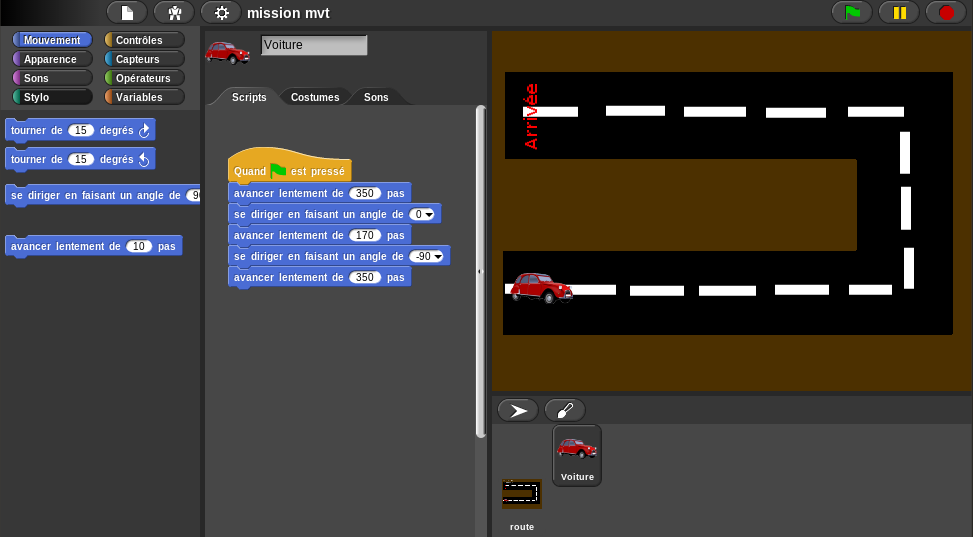
\includegraphics[scale=0.35]{content/7-solution/1-missions/images/voiture}
    \caption{Mission de la voiture}
    \label{fig:mission-voiture}
  \end{center}
\end{figure}


\subsection{L'hélicoptère}
Pour cette mission, voir figure \ref{fig:mission-hélicoptère}, les participants étaient aux commandes d'un hélicoptère. Leur but est de faire le tour de la piste. La piste est un ellipsoïde border d'herbe. Si l'hélicoptère touche l'herbe, il explose et comme pour le précédent, à chaque lancement de scripte l'hélicoptère se repositionnait à son point de départ. Ceci toujours dans le but de forcer les participants à voir la solution dans son ensemble et non juste a la prochaine étape. En plus, l'herbe et de la piste, sur le contour extérieur de la piste est positionner une bande rouge et à l'intérieur elle est bleu. Le but est de tournée des qu'une de ces deux couleurs est touchée et ce pour évité l'herbe.\\

Les concepts introduits par cette mission sont :
\begin{itemize}
\item les boucles, particulièrement le \texttt{while} ;
\item la gestion des collisions grâce au capteur de couleur ;
\item la division en sous process (un pour avancer, un pour la collision rouge et un pour la bleu).
\end{itemize}
\begin{figure}[ht]
  \begin{center}
    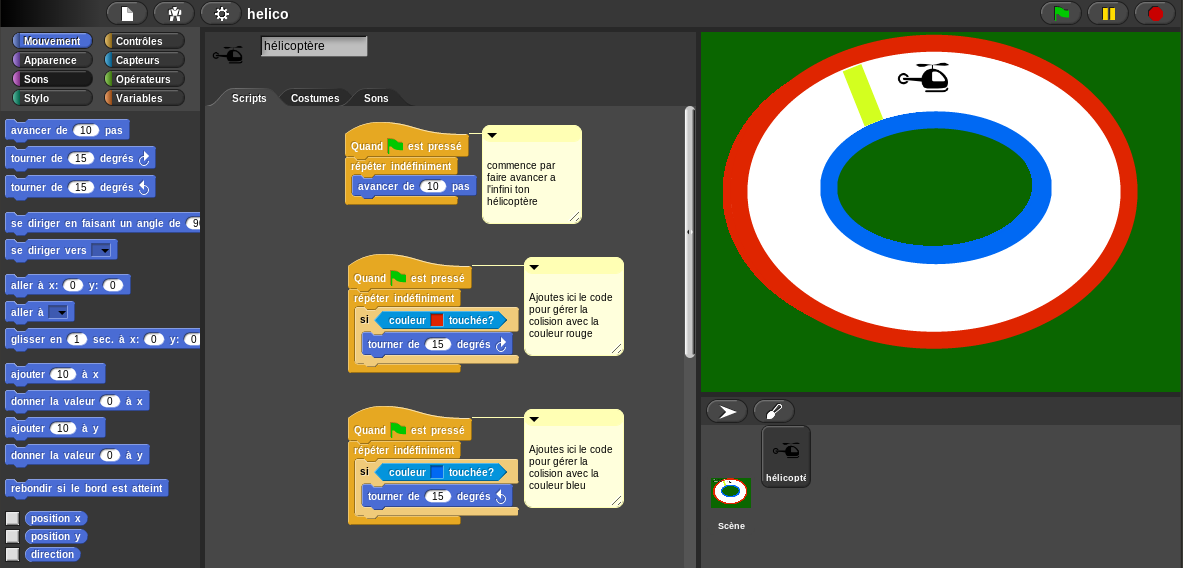
\includegraphics[scale=0.3]{content/7-solution/1-missions/images/helicoptere}
    \caption{Mission de l'hélicoptère}
    \label{fig:mission-hélicoptère}
  \end{center}
\end{figure}

\subsection{Soyons courtois}
Dans cette dernière mission de préparation, voir figure \ref{fig:courtois}, les participants se retrouvent à diriger un personnage qui croise d'autres personnages. Ces derniers disent bonjour à chaque qu'ils croisent quelqu'un. Le but de la mission est dire bonjour également quand le personnage du participant croise quelqu'un.

Les concepts introduits par cette mission sont :
\begin{itemize}
\item la gestion des collisions grâce au capteur de sprite ;
\item la division en sous process (un pour chaque personne) ;
\item Introduction à l'interactivité de l'interface (faire déplacer un personnage) ;
\item la gestion des dialogues et affichage de texte.
\end{itemize}
\begin{figure}[ht]
  \begin{center}
    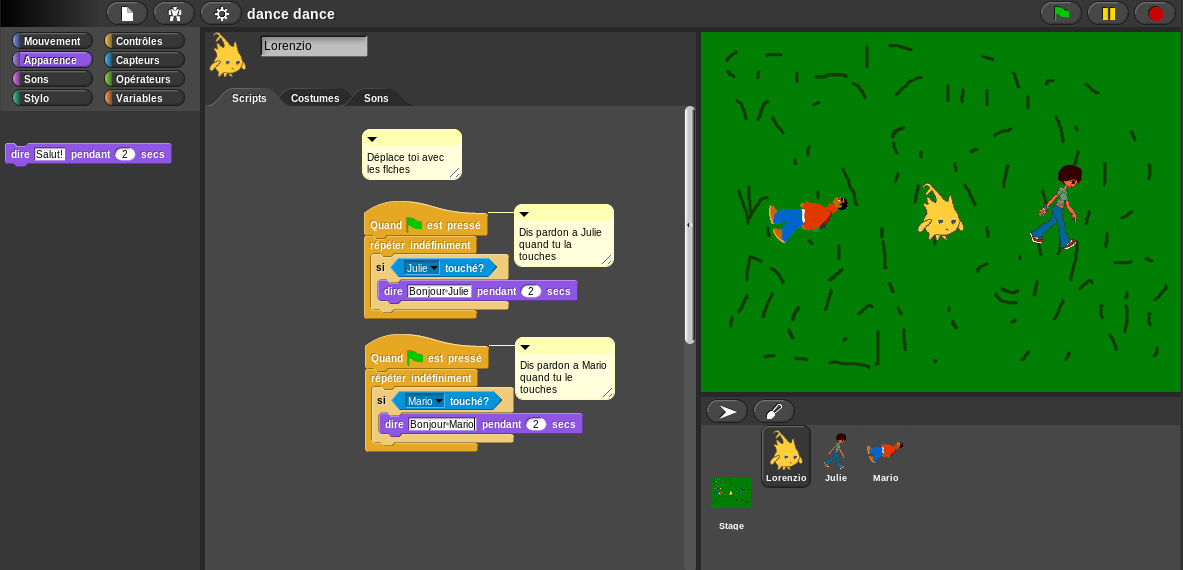
\includegraphics[scale=0.3]{content/7-solution/1-missions/images/courtois}
    \caption{Mission de soyons courtois}
    \label{fig:courtois}
  \end{center}
\end{figure}
\subsection{Chien et chat}
\label{chien-chat}
Cette mission est la dernière de la série et a pour but de mettre ensemble tous les concepts vus dans les missions de préparations. Dans cette mission les étudiants doivent faire en sorte d'avoir deux personnages et de pouvoir les déplacer séparément à l'aide des touches. Le chien doit courir après le chat. Si celui-ci est touché par le chien il crie et le chien gagne un point.\\

Cette mission reprend les concepts vus dans les missions de préparation au quels il faut ajouter:
\begin{itemize}
\item la gestion des variables à travers la variable de score ;
\item l'activation d'un script sur un événement pour les déplacements ;
\end{itemize}

Pour les déplacements, il est déjà présent dans la mission précédente, mais à l'état passif. Ils ne font que l'utiliser, ils ne l'ont pas crée eux-mêmes. Dans cette mission, ils doivent le faire tout seuls. Ceci permet de bien fixer ce concept qui est important dès qu'une interaction clavier est souhaitée.

%analyse mission voiture, cela à permis de prendre en main les entrées des blocs. Au début, beaucoup prennent 3 blocs avancer de 10 pas pour faire 30 pas au lieu de changer la valeur du 10 en 30.

\section{Snap!}
\label{solution SNAP}
Comme expliqué précédemment, nous sommes partis d'un projet existant, Snap! BYOB, pour l'environnement de programmation. Ce projet a pour but de fournir une interface et un environnement supportant la programmation par bloc. Ce projet ne s'inscrit pas dans le cadre d'un apprentissage scolaire ou guidé. Il a donc fallu adapter le projet pour une utilisation plus scolaire. Nous allons expliquer dans cette partie les différentes adaptations que nous avons apportées au projet d'origine et pourquoi elles sont nécessaire pour remplir nos objectifs.\\

Dans les adaptations opérées, nous retiendrons : une simplification de l'interface, la sauvegarde sur les serveurs du projet courant, une différenciation de rôle pour le professeur par rapport au public cible, une amélioration de la traduction en français, le masquage des scripts.

\subsection{L'interface}
\label{interface}
Comme expliqué précédemment le projet original n'avait pas une vocation didactique de groupe et avait un publique cible plus large que le notre. Dans cette idée, il y avait des menus pour des fonctionnalités de gestion de l'ordonnanceur, option d'affichage, paramètres d'éditions, etc. Il est évident que ces fonctionnalités ne sont pas utiles pour notre public. De plus vu l'âge de notre public toutes distractions qui peuvent être évitées améliorent sensiblement l'attention de ces dernier.

Dans cette optique, nous avons opéré un nettoyage en profondeur de l'interface dans l'optique de laisser uniquement les menus utiles. Toutefois comme il est discuté dans les rôles \ref{role}, il est intéressant de ne pas simplement les effacer, mais bien de les masquer.\\

Une autre adaptation de l'interface réalisée est l'ajout d'un menu pour les interactions avec notre plateforme web. Ce menu contient des boutons tel que : "sauvegarder sur le serveur" pour enregistrer leur travail sur la plateforme; "description" qui permet de retrouver le résumé introductif de la mission; "retour à la liste des missions" qui demande a sauver le travail puis renvoi vers la page listant les missions sur le site web.

\subsection{Les rôle}
\label{role}
Dans l'optique de fournir une interface épuré pour les étudiants comme expliqué dans la section \ref{interface}. Il était nécessaire d'enlever des parties de l'interface non pertinente. Toutefois, ces options inutiles aux étudiant peuvent l'être pour les professeurs, mais également pour une missions en "monde ouvert". Il est donc utile de ne pas dédoubler les interfaces mais bien d'avoir une interface modulaire suivant son utilisation. \\

Pour différencier les utilisations de l'interface, nous avons ajouté la notion de rôles. Nous avons défini deux rôle: étudiant et professeur. Grâce à cela, quand les étudiant ouvre un projet, Snap! est lancé avec le rôle étudiant ce qui permet de ne pas afficher les options superflues. Quand c'est un professeur qui souhaite modifier une mission ou en créer une nouvelle, RSNAP lance Snap! avec le rôle professeur ce qui permet d'avoir accès aux fonctions avancées de Snap!.\\

Ces rôles permettent également la gestion du masquage de script. En effet il est intéressant qu'un professeur puisse masquer des blocs, mais cela ne sert à rien si les étudiants peuvent les ré-afficher.

\subsection{Masquer les scripts}
Il a été nécessaire pour la création des missions de cacher des blocs au étudiant. Par exemple la partie de vérification du code de l'étudiant ou encore le code de l'environnement de la mission ne doivent pas apparaître pour les étudiants. 

Une possibilité de cacher des blocs existait déjà dans à partie de gauche de l'interface pour que tout les bloc n'apparaissent pas comme on peut le voir sur la figure \ref{fig:cacher}. Nous avons étendu cette fonction pour pouvoir également cacher des blocs ou des scripts dans la partie d'édition.

Il a également fallu ajouter cette information dans la sauvegarde du projet. Ceci a été réalisé grâce a la balise \texttt{hidden} dans le XML. Cette balise n'est présente que si le bloc doit être caché pour limiter les ajouts au document de sauvegarde.\\

Cette fonctionnalité pouvant être intéressante pour le projet original, elle a été proposé dans une \texttt{pull request}. Les responsables de Snap! ont été très intéressé par cette fonctionnalité qui est toujours en cours d'étude.
\begin{figure}[ht]
  \begin{center}
    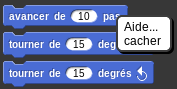
\includegraphics[scale=0.5]{content/7-solution/2-snap/images/cacher}
    \caption{Option pour cacher la définition d'un bloc}
    \label{fig:cacher}
  \end{center}
\end{figure}

\subsection{Traduction}
Le caractère francophone de ce travail est une part importante dans sa différenciation par rapport au autres initiatives similaires introduits dans la section \ref{travail associé}. L'application était déjà traduite partiellement en français mais une large majorité des traduction étaient incomplètes, inexistante ou erronée. Une partie du travail a donc été de finir et amélioré la traduction de l'application. La traduction de l'application se divise en deux partie, la partie interface et la partie aide. Pour ce travail a été développé des outils de traduction d'aide automatisé. Ces outils ont été développé car des aide en français existait déjà dans le projet SCRATCH. Il était donc plus efficace d'avoir un outils de traduction automatique que de retraduire manuellement les aides.

Cette partie a été proposée au projet original de Snap! et acceptée mais ne sera intégré qu'après quelques aménagements. Elle est donc actuellement acceptée mais en attente.

\subsection{Sauvegarde sur le serveur}
Comme il était nécessaire d'interfacé l'environnement de programmation avec un site web, nous avons du reimplementer certaine fonctionnalité d'import-export.\\

Il était nécessaire de disposer d'un fichier XML pour le sauvegarder sur les serveurs. Des fonctions existantes ont été adapté pour permettre d'avoir ce fichier et de pouvoir l'envoyer sur l'adresse internet désirée.


\section{Rsnap}
\graphicspath{{content/7-solution/3-rsnap/images/}}

\subsection{Interface}
présentation de l'interface :
\begin{itemize}
  \item design joli et adaptative
  \item student side
  \item prof side
  \item arrangement des missions + ouverture successive
  \item passage rsnap/snap
\end{itemize}

\subsection{Implémentation}
Comme expliqués en section \ref{rails}, Rails possède une architecture Model-Vue-Controleur (MVC). Cette section va présenter l'application en se basant sur ce modèle d'architecture. La première expliquera donc le modèle, ensuite les contrôleurs seront discutés et enfin les vues seront présentées.

\subsubsection{Modèles}
Les différents concepts utiles pour développer l'application sont ceux représentés par les différents modèles. Ceux-ci sont présentés sur la figure \ref{fig:models}.

\begin{figure}
 \begin{center}
   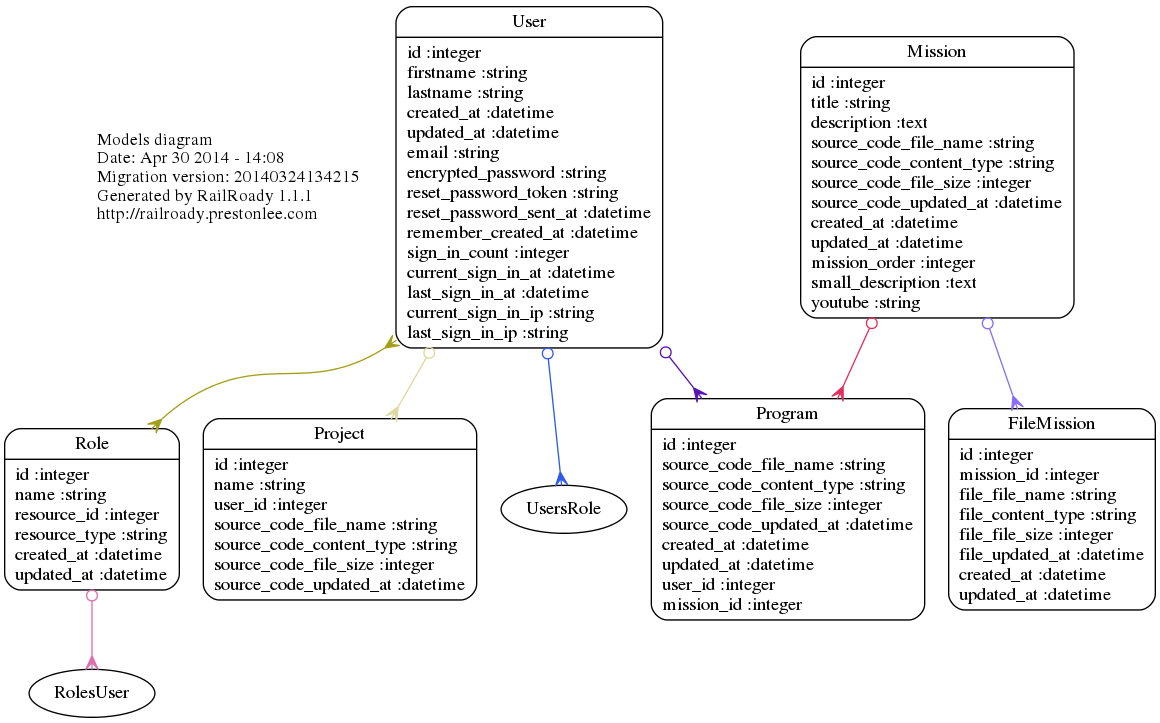
\includegraphics[width=\textwidth]{models_complete}
   \caption{Modèles de Rsnap}
   \label{fig:models}
 \end{center}
\end{figure}

\paragraph{\texttt{User}} L'utilisateur contient les informations nécessaires à le représenter (\texttt{firstname}, \texttt{email} \ldots) et les informations pour s'authentifier (\texttt{encrypted\_password}, \texttt{current\_sign\_in\_ip}, \ldots). L'utilisateur peut posséder plusieurs rôles, programmes et projets.

\paragraph{\texttt{Rôle}} Les rôles permettent de donner des attributs à un utilisateur. Ce modèle a été généré automatiquement par Rolify \ref{rolify}. Dans le cas de Rsnap, deux rôles ont été créés : \texttt{admin} et \texttt{teacher}. Ces deux rôles sont globaux et donc ne sont pas rattachés à une ressource spécifique.%TODO dans futur Works: role teacher sur ressource students_group

Les rôles seront utiles en conjonction avec les autorités \ref{authority} pour donner des droits supplémentaires à ces types d'utilisateurs.

\paragraph{\texttt{Mission}} Les missions représentent tout ce qui est nécessaire pour avoir un exercice. Une mission comporte donc un titre, une description avec des images et une vidéo pour expliquer à l'étudiant ce qu'il devra faire. Elle comporte en plus le code source initial de l'exercice. Généralement, celui-ci contient le squelette initial du programme pour l'étudiant et les tests pour vérifier le programme. 

\paragraph{\texttt{FileMission}} Les fichiers liés à une mission sont les différentes images que compose la description. %TODO dans furture work : on peut imaginer rajouter la possibilité de mettre d'autre style de fichier dedans : ex. PDF, slide de cours...

\paragraph{\texttt{Program}} Les programmes comportent la solution d'un étudiant à une mission donnée. Ils comportent uniquement le code source de l'étudiant.

\paragraph{\texttt{Project}} Les projets sont identiques aux programmes excepté qu'ils ne sont pas liés à une mission. Ils comportent donc le nom du projet en plus du code source.

\paragraph{Exemple} \texttt{Program} est un bon exemple de modèle Rails (code source \ref{lst:model-program}). Seules les fonctionnalités qu’Active Record \ref{active-record} ne sait pas déduire de lui-même sont présentes. Le modèle contient donc uniquement :
\begin{itemize}
  \item le nom des modèles avec qui il est associé et la cardinalité de la relation (\texttt{belong\_to}) ;
  \item la validation de certains attributs pour qu'ils respectent certaines contraintes (\texttt{validate}) ;
  \item des méthodes de classes pour simplifier les requêtes au modèle (\texttt{scope}, \texttt{self.*}).
\end{itemize}

Comme c'est visible dans les \texttt{scope}, Active Record permet de faire des requêtes SQL directement en Ruby. 
\lstinputlisting[language=Rails, firstline=21, caption={Modèle \texttt{Program}}, label=lst:model-program]{content/7-solution/3-rsnap/listings/program.rb}

\subsubsection{Controlleurs}
Les contrôleurs donnent accès à différentes ressources. La figure \ref{fig:controllers} montre la liste des contrôleurs implémentés pour l'application. La majorité de ceux-ci se rapporte directement à un modèle spécifique. Il existe néanmoins certaines ressources différentes telles que : 
\begin{itemize}
  \item les pages statiques (\texttt{HomeController}) ;
  \item l'ordonnancement des missions (\texttt{SortMissionsController}) ; 
  \item la création d'un programme depuis une mission (\texttt{InitializationMissionController}) ;
  \item les ressources utiles à l'affichage de Snap! (\texttt{SnapAssetsController}).
\end{itemize}
\begin{figure}
 \begin{center}
   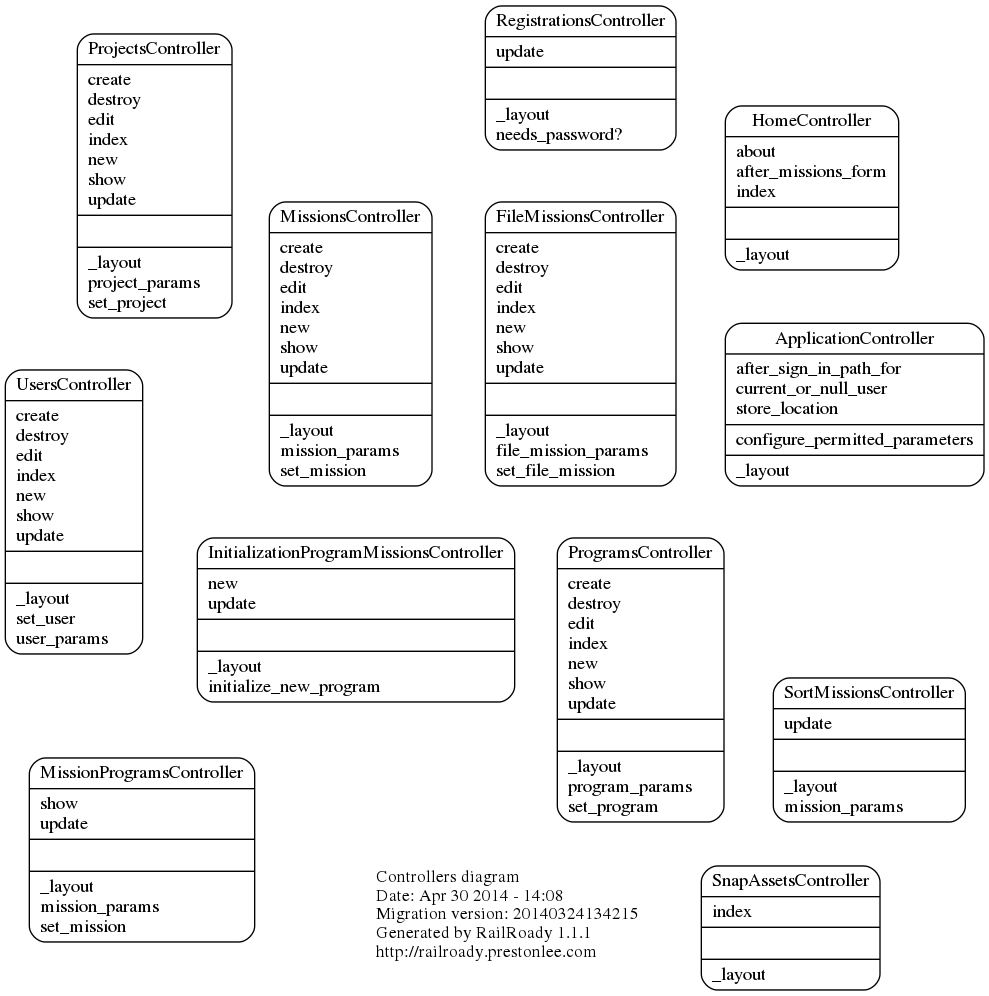
\includegraphics[width=\textwidth]{controllers_complete}
   \caption{Controlleurs de Rsnap}
   \label{fig:controllers}
 \end{center}
\end{figure}

Comme expliqué dans la section \ref{controleur}, les méthodes accessibles sont définies dans \texttt{routes.rb}. Les contrôleurs ont des tous des ressources RESTfull exceptées \texttt{HomeController}. Ceci est visible dans \texttt{routes.rb} ou en regardant les fonctions publiques disponibles dans les contrôleurs sur la figure \ref{fig:controllers}.

\paragraph{Exemple}
L'extrait du contrôleur \texttt{MissionsController} \ref{lst:controller-mission} montre l'usage classique d'un contrôleur. 

\lstinputlisting[language=Rails, linerange={1-5,10-34,52-62}, caption={Extrait du controlleur \texttt{MissionsController}}, label=lst:controller-mission]{content/7-solution/3-rsnap/listings/missions_controller.rb} %TODO verifier les ranges des lignes

Grâce au méta-programmation, \lstinline[language=Rails]{authorize_actions_for Mission} permet de rajouter, sur toutes les méthodes RESTfull, une vérification de ce que peut réaliser ou pas l'utilisateur courant. Ces vérifications sont déportées dans les autorités \ref{autority}. De plus, la méthode \lstinline[language=Rails]{before_filter} permet de réaliser une action supplémentaire avant chaque appel de fonction. Ici, excepté pour l'action \texttt{show} et \texttt{index} qui peuvent être publique, il faut que l'utilisateur soit authentifié pour que l'application puisse par après vérifier ses droits. %TODO pas claire sur la fin tu commences par les exceptions

Dans une méthode du contrôleur accessible via les routes, plusieurs actions sont à réaliser :
\begin{enumerate}
  \item traiter si nécessaire les paramètres fournis. Ceux-ci se trouvent dans \lstinline[language=Rails]{param} ;
  \item Assigner les variables d'instance que nécessitera la vue pour s'afficher correctement ;
  \item Exécuter le rendu de la page. Si la vue a le même nom que la méthode, cette étape est facultative.
\end{enumerate}

\subsubsection{Vue}
\label{vues}
Les vues sont écrites en haml \ref{haml}. L'exemple de code \ref{lst:vue-user-index} avec \ref{lst:vue-user-partial} montre comment est représenté la vue servant à lister tout les utilisateurs \ref{fig:vue-users}.

\lstinputlisting[language=haml, caption={Vue \texttt{index} des utilisateurs}, label=lst:vue-user-index]{content/7-solution/3-rsnap/listings/index.html.haml}
Le code source \ref{lst:vue-user-index} présente comment sont utilisé les variables d'instance créées par le contrôleur. Par exemple, la variable \texttt{@title} sert de titre 1.

\lstinputlisting[language=haml, caption={Vue d'une ligne \texttt{\_user} représentant un utilisateur}, label=lst:vue-user-partial]{content/7-solution/3-rsnap/listings/_user.html.haml}
De plus, Rails permet de faire le rendu d'un autre fichier de manière élégante. La ligne 14 du code source \ref{lst:vue-user-index} permet d'exécuter le rendu sur tous les éléments de la collection \texttt{users} grâce au fichier \ref{lst:vue-user-partial}

Les connaisseurs de Bootstrap \ref{bootstrap} auront reconnu l'usage intensif des classes de style qu'il propose. L'adaptativité de cet outil est visible sur la capture d'écran \ref{fig:vue-users}. En effet, le menu supérieur a été réduit, car la taille de l'écran était trop petite pour accueillir le menu en entier.

\begin{figure}
  \begin{center}
    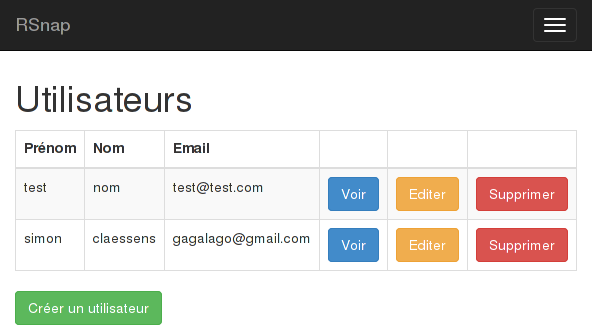
\includegraphics[width=.8\textwidth]{users}
    \caption{Affichage de la vue présentée par le code source \ref{lst:vue-user-index} et \ref{lst:vue-user-partial}}
    \label{fig:vue-users}
  \end{center}
\end{figure}

\subsection{Choix techniques}
expliquer les différentes possibilités de stockage (fichier et site) prix, fonctionnalité...

\subsection{Utilisation}
Pour utiliser la plateforme, il faut tout d'abord s'enregistrer dessus. Ensuite, suivant le profil, différentes actions sont possibles. L'utilisateur normal peut uniquement résoudre les missions dans l'ordre proposé par les professeurs. Les professeurs peuvent aussi créer des missions. Cette section va présenter l'utilisation de la plateforme.
%TODO faire des schémas/scénario avec les screenshot + tous les screenshot en annexe

\paragraph{Professeur}
Un professeur pour réaliser un cours de programmation doit pouvoir faire les choses suivante:\\
\begin{description}
  \item[Créer des missions] Pour créer une nouvelle mission, le professeur doit se rendre sur la page qui liste toutes les missions (figure : \ref{fig:mission-order}), ensuite il peut cliquer sur le bouton en bas de page "Nouvelle mission". La page suivante (figure: \ref{fig:create-mission}) permet de renseigner les informations sur la mission : titre, description et explication de la mission, vidéo d'explication \ldots Il reste enfin à créer la mission proprement dite. Pour cela, lorsque le professeur clique sur le bouton "Créer une mission", il est redirigé vers l'interface de Snap! (figure : \ref{fig:snap-menu}). Il peut alors créer tout ce qui est nécessaire à la réalisation et au test de la mission. Avant de sauver, il ne doit pas oublier de cacher les blocs et les scriptes qui ne doivent pas être visibles aux étudiants.
  \item[Ordonner les missions] Pour ordonner les missions dans un ordre pédagogique, il suffit de glisser les missions dans la liste (figure : \ref{fig:mission-order})
  \item[Corriger les soumissions de ses étudiants] Pour corriger les soumissions de ses étudiants, le professeur doit simplement se rendre sur la page des programmes (figure : \ref{fig:program-list}). À ce moment, le professeur peut simplement voir le programme qu'il désire corriger et rajouter des commentaires dans l'interface de Snap! (figure : \ref{fig:snap-menu}) qui s’ouvrira avec le programme de l'étudiant.
\end{description}

\paragraph{Étudiant}
Un étudiant veux pouvoir réaliser les opérations suivantes :
\begin{description}
  \item[Réaliser une mission] L'étudiant peut réaliser une mission en cliquant sur le nom de la mission. Soit il continue la mission là où il l'a laissée si le bouton est bleu, soit il commence la dernière mission qui lui est accessible. Dans les deux cas, il se retrouve sur l'interface de Snap! où il peut résoudre la mission.
  \item[Réaliser un projet libre] Si l'étudiant a envie de créer quelque chose, il peut aller dans projet libre. Il aura alors à disposition le plein potentiel de Snap! et pourra laisser libre court à son imagination pour créer le programme de ses rêves.
\end{description}

\begin{figure}
  \begin{center}
    
\includegraphics[width=\textwidth]{snap.png}
    \caption{Réalisation d'une mission}
    \label{fig:snap-menu}
  \end{center}
\end{figure}
\begin{figure}
  \begin{center}
    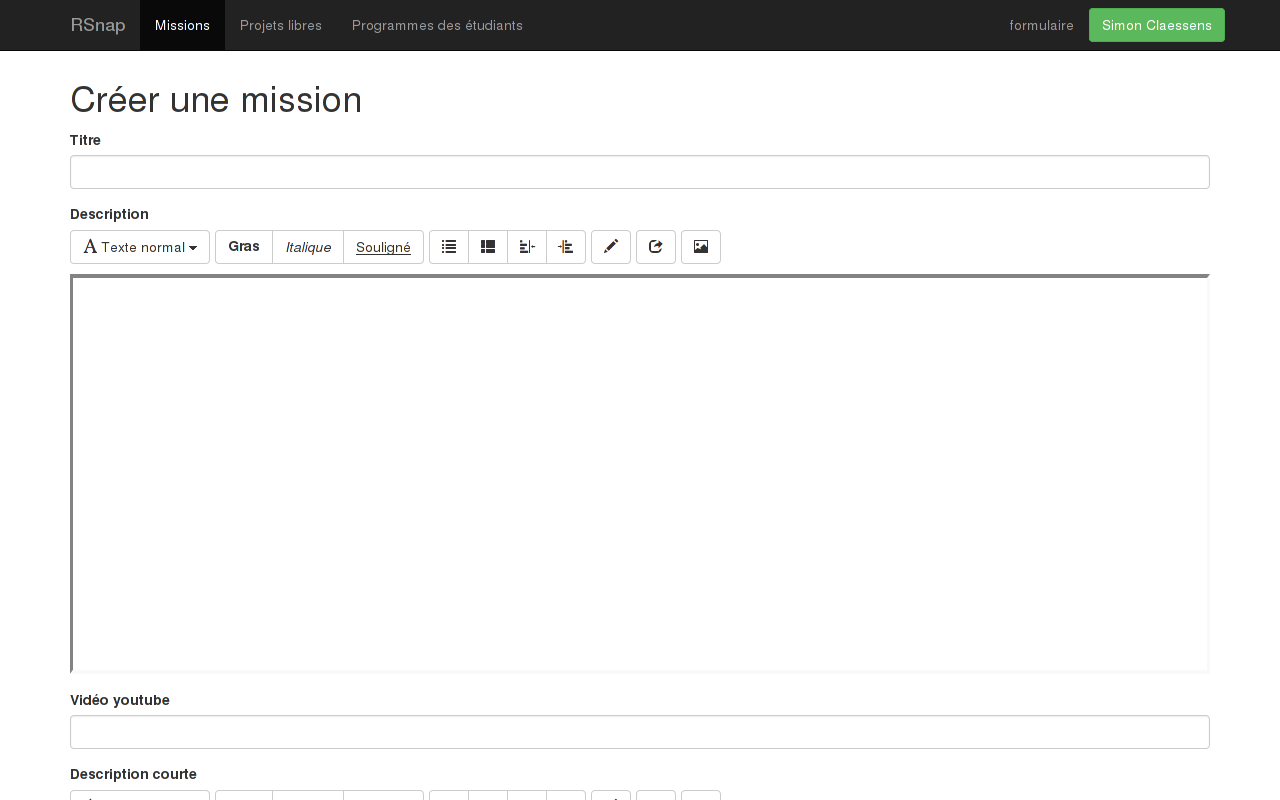
\includegraphics[width=\textwidth]{create-mission.png}
    \caption{Création d'une mission}
    \label{fig:create-mission}
  \end{center}
\end{figure}
\begin{figure}
  \begin{center}
    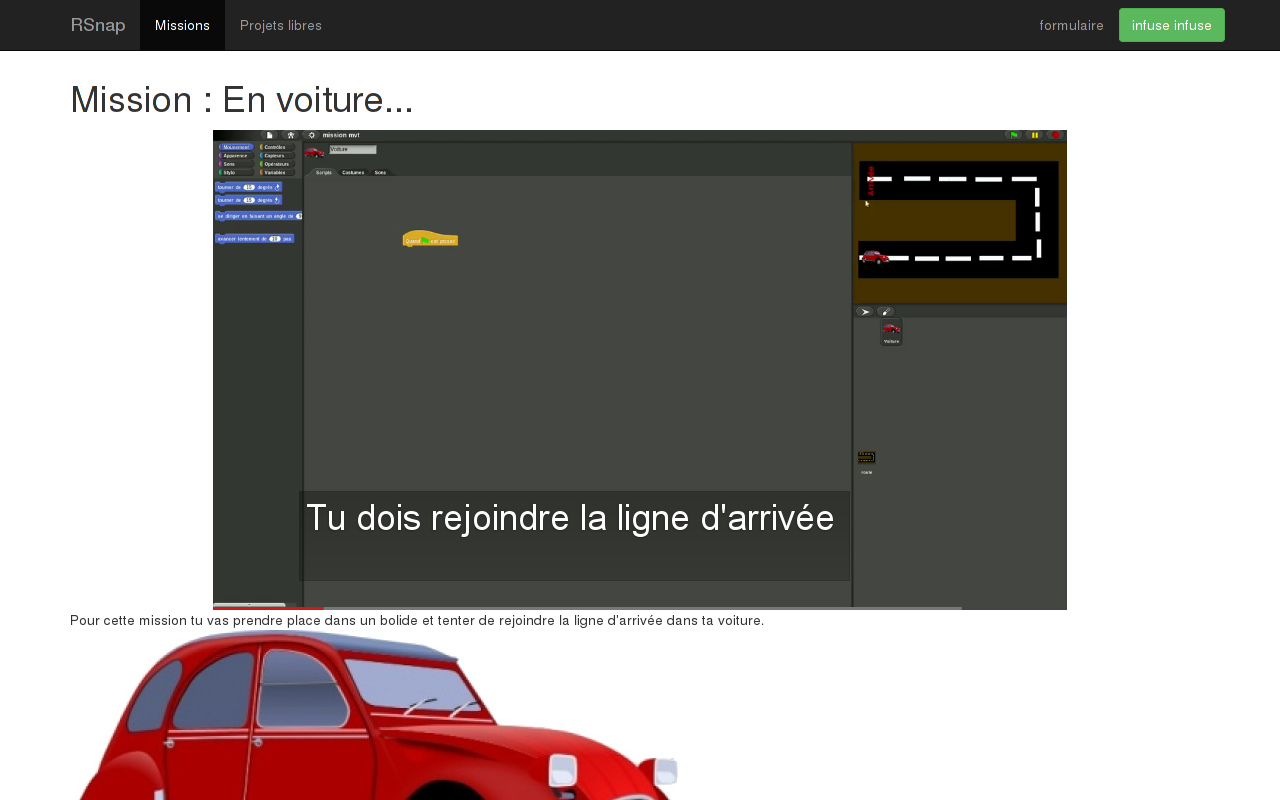
\includegraphics[width=\textwidth]{mission-description.png}
    \caption{Description d'une mission}
    \label{fig:mission-description}
  \end{center}
\end{figure}
\begin{figure}
  \begin{center}
    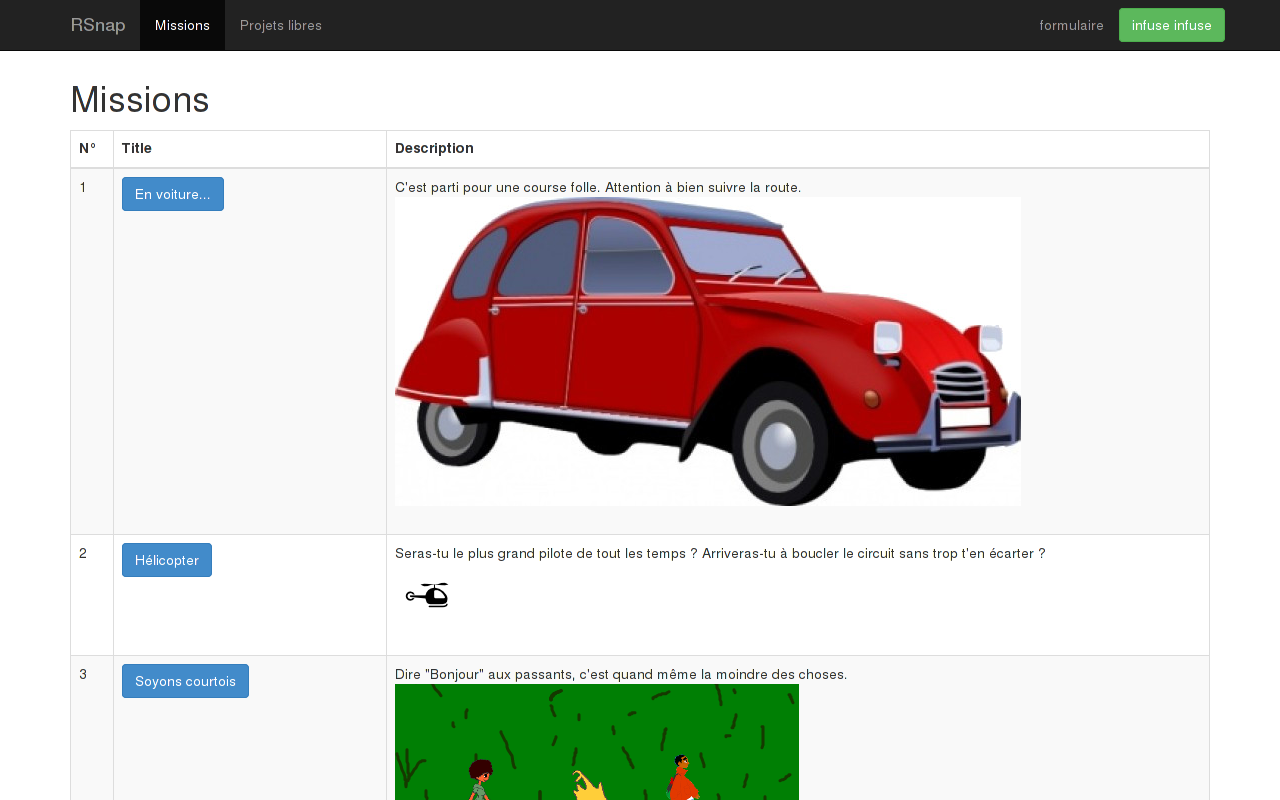
\includegraphics[width=\textwidth]{mission-list-student.png}
    \caption{Liste des missions accessible par un étudiant}
    \label{fig:mission-list-student}
  \end{center}
\end{figure}
\begin{figure}
  \begin{center}
    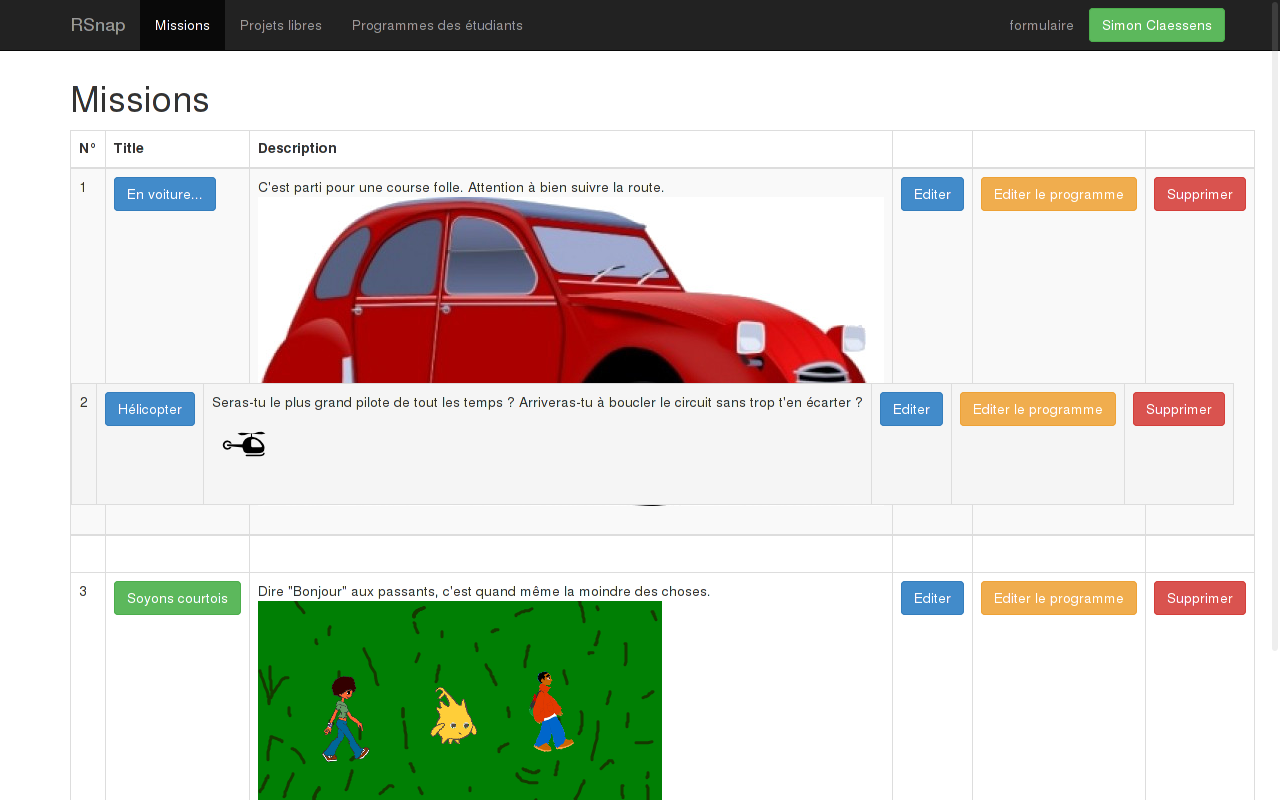
\includegraphics[width=\textwidth]{mission-order.png}
    \caption{Liste des missions vue par un professeur durant un ordonancement}
    \label{fig:mission-order}
  \end{center}
\end{figure}
\begin{figure}
  \begin{center}
    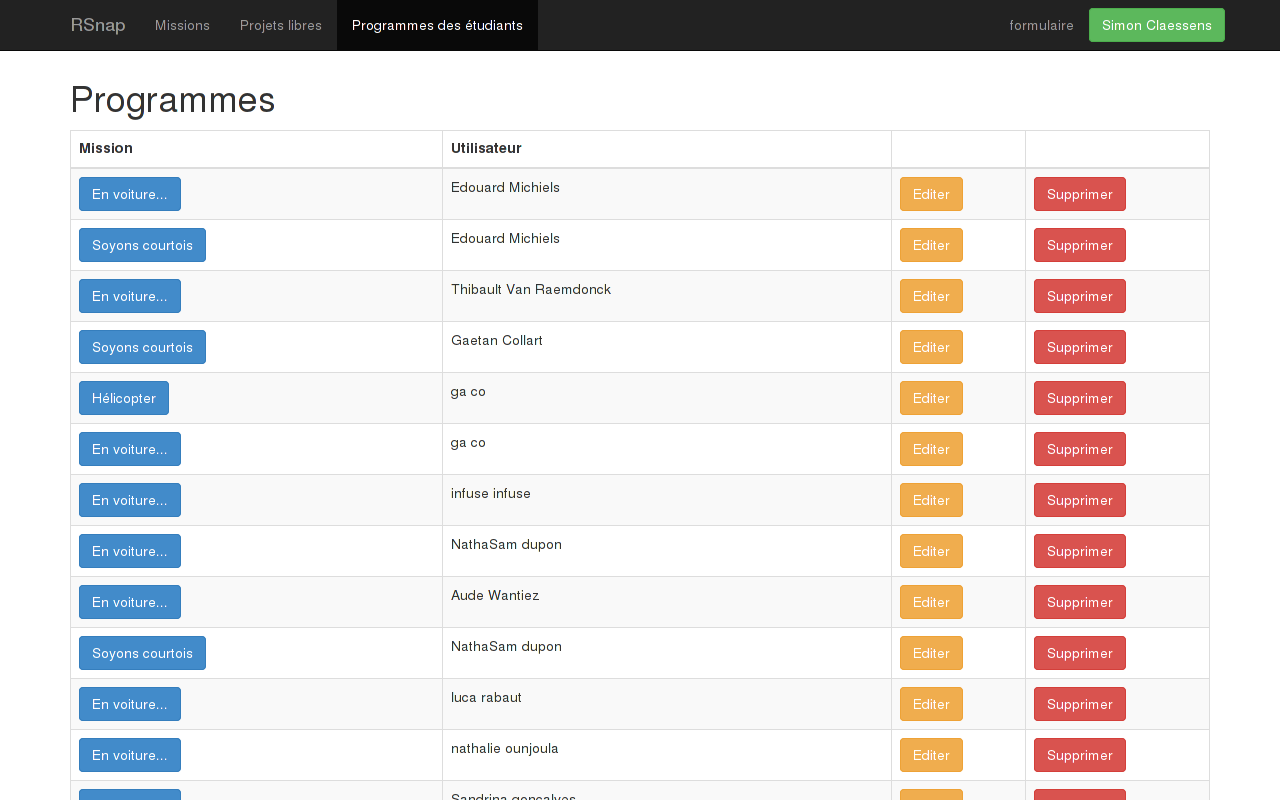
\includegraphics[width=\textwidth]{program-list.png}
    \caption{Liste des programmes visible par un professeur}
    \label{fig:program-list}
  \end{center}
\end{figure}
\begin{figure}
  \begin{center}
    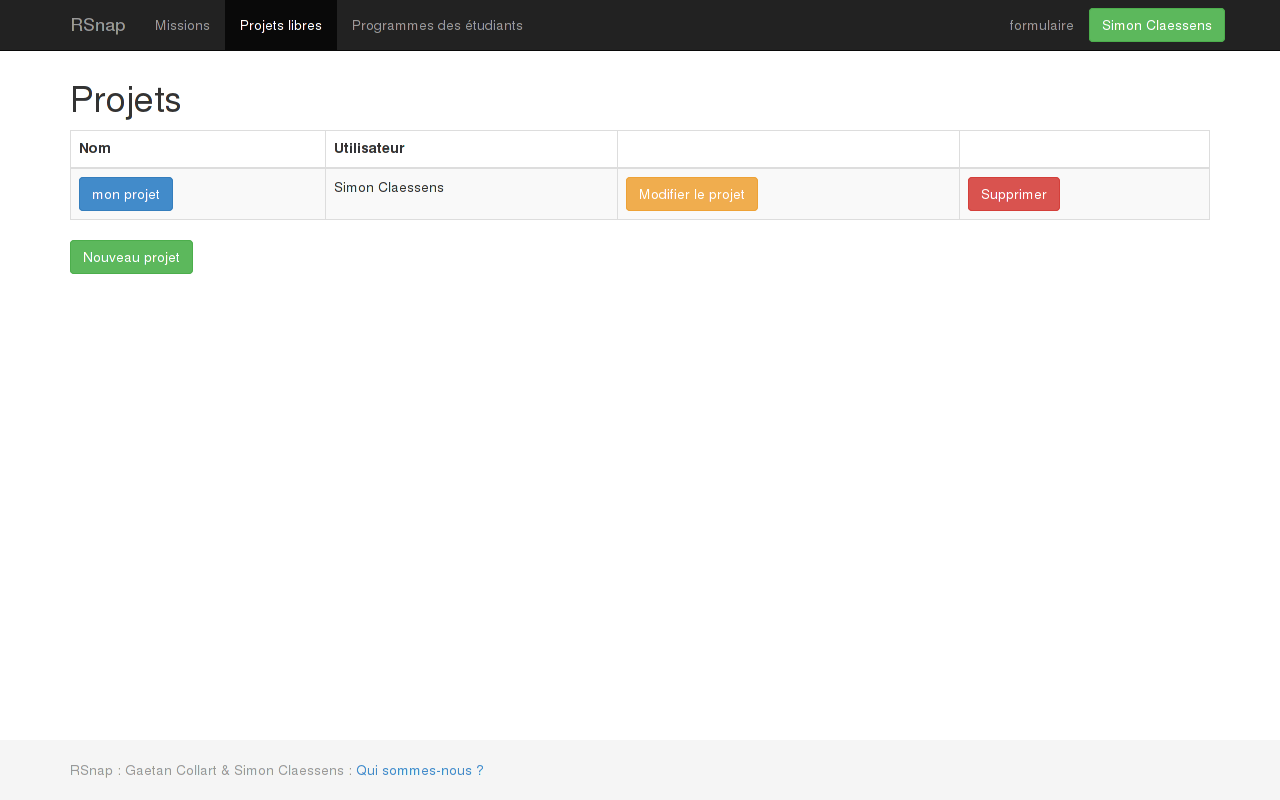
\includegraphics[width=\textwidth]{project-list.png}
    \caption{Liste des projets libres d'un utilisateur}
    \label{fig:project-list}
  \end{center}
\end{figure}


\paragraph{Choisir mission}

\paragraph{Voir intro mission}

\paragraph{Réaliser mission} voir plus haut dans la description des missions les screeenshot ont déjà été montré, mais rajouter la vue du menu robot

\paragraph{Projet libre}
Expliquer que c'est la mm chose que les missions, mais sans passer par la case description.

\paragraph{créer mission}

\paragraph{administrer mission étudiante} montrer la vue qui liste tout les programme

\paragraph{ordonancer mission}

%\include{content/scopj/scopj}
%\include{content/scopj/implementation}
%\include{content/scopj/threading}


%==========================
%       PART 3
%==========================
\chapter{Conclusions}

\chapter{Future amélioration}

%\chapter{Référence}

%\include{content/cityvisit/cityvisit}
%\include{content/efficiency/efficiency}
%\include{content/conclusion/futurework}
%\chapter{Conclusions}



% \appendix
% \glsaddall
% \printindex
% \printglossaries
% %\include{content/cityvisit/data}
% \nocite{*}
% \bibliographystyle{alpha}
% \bibliography{biblio}

%\printnomenclature
%\cleardoublepage


\end{document}
